\chapter{Damage}
\label{chap:damage}
Each Attack reduces the opponent's Hit Points by some positive integer.
This integer is called (inflicted) damage $D$, and calculated as a product of several factors.
The factors are different for Gym/Raid/Max Battles and Trainer Battles,
 but the core of the damage equation is common to all contexts.

\section{The typing multiplier}
\label{sec:typemult}
Determine $M_C$, the common multiplier due typing:

\[ M_C = M_{STAB} \times 1.6^{T} \]

$M_{STAB}$ is the STAB bonus, equal to 1.2 when the Attack's Type matches any
  Type of the attacker, and 1 otherwise.
$T$ is the number calculated in \autoref{chap:types} using the Attack Type
 and the defender's Type.
I have included a $T$ of -4 in \autoref{table:typemult} for completeness,
 but remember that this is not currently realizable.

\begin{table}
\begin{center}
\begin{tabular}{c r r r r}
  $T$ & $1.6^{T}$ & Δ\% & w/ STAB & Δ\% \\
\Midrule
  -4 & 0.1526 & -84.74 & 0.1831 & -81.69 \\
  -3 & 0.2441 & -75.59 & 0.2930 & -70.7 \\
  -2 & 0.3906 & -60.94 & 0.4688 & -53.12 \\
  -1 & 0.625 & -37.5 & 0.75 & -25 \\
  0 & 1 & 0 & 1.2 & 20 \\
  1 & 1.6 & 60 & 1.92 & 92 \\
  2 & 2.56 & 156 & 3.072 & 207.2 \\
\end{tabular}
\caption{Typing multipliers with and without STAB}
\label{table:typemult}
\end{center}
\end{table}

Leaving out the hideous −4 case, we see that $M_C$ ranges
 from 0.2441 (a 75.59\% reduction in damage) to 3.072
 (a 207.2\% increase).
Considered another way, for an effectiveness of −3 with no STAB bonus,
 it takes about four times as many Attacks to subdue an opponent than
 we would otherwise expect.
With an effectiveness of 2 with STAB, it takes about one-third as many Attacks.

Note that the change due to a $T$ of 1 (60\%) is similar in magnitude to the change
 when $T$ is -2 (-60.94\%). A $T$ of -1 is a smaller loss (-37.5\%).
This does not mean that an Attack ineffective against one of the defender's types and
 effective against the other enjoys a 22.5\% gain (as one would see from $1.6^{-1} + 1.6^{1})$!
The multiplier is 1, and results in no change ($1.6^{-1+1}$).
The two effectiveness relationships must be added, and this value used to
 calculate $1.6^T$.
Exponential functions are not linear functions, and must not be treated as such.

\section{The context-specific multiplier}
\label{sec:mbmult}
In Raids and Max battles, a number of effects come into play.
\[ M_B = 0.5 \times M_D \times M_F \times M_W \times M_M \]
\begin{itemize}
 \item $M_D$ is 0.25 if the Attack is dodged (dodging is only possible in Raids/Max battles),
 and 1 otherwise. Note that this seems to have been subject to recent changes.
 \item The friendship bonus $M_F$:
   \begin{table}[h!]
     \begin{center}
       \begin{tabular}{lc}
         Situation & $M_F$ \\
         \Midrule
         No friends present, \textit{unless…} & 1 \\
         Battling with at least one Good Friend, \textit{unless…} & 1.03 \\
         Battling with at least one Great Friend, \textit{unless…}  & 1.05 \\
         Battling with at least one Ultra Friend, \textit{unless…} & 1.07 \\
         Battling with at least one Best Friend. & 1.1
       \end{tabular}
     \end{center}
     \caption{Bonus due the presence of friends}
   \end{table}
 \item $M_W$ is 1.2 if the Attack is weather-boosted, and 1 otherwise.
 \item $M_M$ from Mega Pokémon \textit{actively} involved in a Raid (i.e. they
   must be fighting, not just on the team), or Primal Pokémon \textit{present}
   (even knocked out) at a Raid or Gym. The Primal bonus is not awarded to the Trainer who brought
   that Primal Pokémon, but they can receive it from some other Trainer's Pokémon.
   \begin{table}[h!]
     \begin{center}
       \begin{tabular}{p{.7\textwidth}c}
         Situation & $M_M$ \\
         \Midrule
         No active Mega Pokémon, and no Primal Pokémon brought
          by other Trainers present, \textit{unless…} & 1 \\
         Battling with at least one Mega Pokémon,
          or another Trainer's Primal Pokémon present, \textit{unless…} & 1.1 \\
         Battling with at least one Mega Pokémon of the attack's type,
          or another Trainer's Primal Pokémon is present and of
          the attack's type. & 1.3 \\
       \end{tabular}
     \end{center}
     \caption{Bonus due the presence of Mega and Primal Pokémon}
   \end{table}
   In a Max battle, $M_M$ is based on the number of Pokémon left at that Power Stop
     (see \autoref{sec:maxbattles}).
   \begin{table}[h!]
     \begin{center}
       \begin{tabular}{lc}
         Pokémon present at Power Stop & $M_M$ \\
         \Midrule
         0 & 1 \\
         1 & 1.1 \\
         2--3 & 1.15 \\
         4--14 & 1.188 \\
         15+ & 1.2 \\
       \end{tabular}
     \end{center}
     \caption{Bonus in Max battles due Pokémon at Power Stop}
   \end{table}
\end{itemize}
The calculation for Trainer Battles is simpler:
\[ M_B = 0.65 \times M_G \]
For Fast Attacks, $M_G$ is 1.
When throwing a Charged Attack, the attacking Trainer plays a short minigame.
Performance on this minigame is summarized with ``Excellent!'', ``Great!'',
``Nice!'', or silence.
This summary typically determines $M_G$, with a range over [0.25, 1].
``Excellent!'' is necessary and sufficient for a 1, and should always be obtainable.
\begin{table}
  \begin{center}
    \begin{tabular}{l r}
      Summary & $M_G$ range (no Shield) \\
      \Midrule
      ``Excellent!'' & 1 \\
      ``Great!'' & [0.75, 1) \\
      ``Nice!'' & [0.5, 0.75) \\
      No summary & [0.25, 0.5) \\
  \end{tabular}
    \caption{The minigame summary is an indication of $M_G$}
  \end{center}
\end{table}
Each Trainer gets two shields in a battle, each of which can be used
 to block a single Charged Attack.
If a shield is used, $M_G$ is 0, no matter the minigame performance.
The effect is equivalent to raising the defender's DEF to infinity for the
  duration of the Attack.

\section{The damage equation}

$D_A$ is what we can calculate using only the attacker's knowledge, i.e.
 it is that component of $D$ which is independent of the defender.

\[ D_A = P \times Eff_A \times M_{STAB} \times M_B \]

Since this is a product, a proportional increase in any factor leads to
 the same change.
Suppose a Level 12 Pokémon (CPM: 0.4628) with $Mod_A$ of 140 runs
  a Fast Attack with a Power of 10 and no STAB bonus.
The resulting $D_A$ is 421.148.
Increasing Power to 12,
 increasing $Mod_A$ to 168,
 acquiring the STAB bonus,
 or increasing CPM 20\% to 0.55536 (somewhere between Levels 17 and 17.5; this exact change is not possible)
 all yield a 20\% increase in $D_A$, 505.3776.
Note that this is all independent of the opponent.

$D_A$ is divided by $Eff_D$ and scaled by $1.6^T$:

\[ D_D = \frac{D_A}{Eff_D} \times 1.6^T \]

We can recover our defined multipliers:

\[ D_D = P \times \frac{Eff_A}{Eff_D} \times M_C \times M_B \]

Using the definitions of $Eff_A$ and $Eff_D$, this can be rewritten as:

\[ D_D = P \times \frac{Mod_A \times CPM_A}{Mod_D \times CPM_D} \times M_C \times M_B \]

which can of course be rewritten as:

\[ D_D = P \times \frac{Mod_A}{Mod_D} \times \frac{CPM_A}{CPM_D} \times M_C \times M_B \]

A floor function is applied to ensure an integer,
 followed by a min function to ensure at least 1 point of damage is always inflicted:

\[ D = \min{1, \left\lfloor P \times \frac{Eff_A}{Eff_D} \times M_C \times M_B \right\rfloor } \]

If $D$ equals or exceeds the opponent's HP, it will fight no more.

\section{Opponent-independent damage}
We can break the damage equation into those parts dependent
 upon opponents, and those which are independent.
Looking at the damage equation, Power, $Eff_A$, and STAB do not depend
 upon an attacker's opponent.
Likewise $Eff_D$ and MHP for the defender.
The attacker knows neither $Eff_D$ nor MHP, while the defender doesn't know $Eff_A$.
Knowing type effectiveness always requires knowing the opposing typing.
We can thus define an independent core fitness evaluation:

\[ F = Eff_A \times P \times M_{STAB} \times Eff_D \times MHP \]

Note that CPM is implicitly cubed in this function.

Of course, a given Pokémon can generally select from multiple Fast and Charged Attacks,
  knowing up to two of the latter at a given time.
Furthermore, Fast and Charged Attacks are not used in equal ratio (there will
  always be multiple Fast Attacks per Charged Attack), and a Shield can
  nullify a Charged Attack.
How do we define $P$ and $M_{STAB}$?
As only one Fast Attack can be known at a time, it's easy enough to define one
  fitness for each possible Fast Attack, leaving out Charged Attacks for now.
All we need do is normalize the Power of the Fast Attack, using the number of
  Turns it requires.

\[ F = Eff_A \times \frac{P_{Fast}}{T_{Fast}} \times M_{STAB-Fast} \times Eff_D \times Eff_S \]

Integrating Charged Attacks is more complex.
First, we can simply normalize the Charged Attack as we did the Fast Attack,
 determine the number of Fast Attacks necessary to launch it:

\[ N_{Fast} = \lceil\frac{E_{Charged}}{E_{Fast}}\rceil \]

yielding the total Power of a cycle.

\[ TDO = N_{Fast} \times P_{Fast} + P_{Charged} \]

We normalize this by the turns of a full cycle:

\[ F_{cycle} = \frac{TDO}{N_{Fast} \times T_{Fast} + T_{Charged}} \]

There are two turns per second. Multiplying $F_{cycle}$ by two yields a
  stat the community calls Damage Per Second (DPS).

This has several problems, almost all related to Charged Attacks.
It doesn't account for the possibility of knowing two Charged Attacks.
It doesn't account for leftover Energy, which will sometimes be present if
  $E_{Charged}$ is not a multiple of $E_{Fast}$ (i.e. $N_{Fast}$
  might fluctuate from one cycle to the next).
It ignores the possibility that the attacker might not use its Charged Attack
  immediately (and it is often unwise to throw Charged Attacks as quickly as
  possible; see \autoref{chap:strategy}).
Finally, it presumes that the attacker can always get off a full cycle.
In reality, the attacker might be knocked out or substituted long before its
  Charged Attack becomes relevant, or the defender might use a Shield.
It is tempting to ignore Charged Attacks, but when they land, they tend to
  dominate our total inflicted damage\footnote{When a Charged Attack is thrown
  early against a lengthy fast attack, it allows for a ``free fast attack''
  (see \autoref{chap:battle}). This needn't be taken into account, as it is
  technically imperfect play.}.

\begin{figure}[ht]
  \centering
  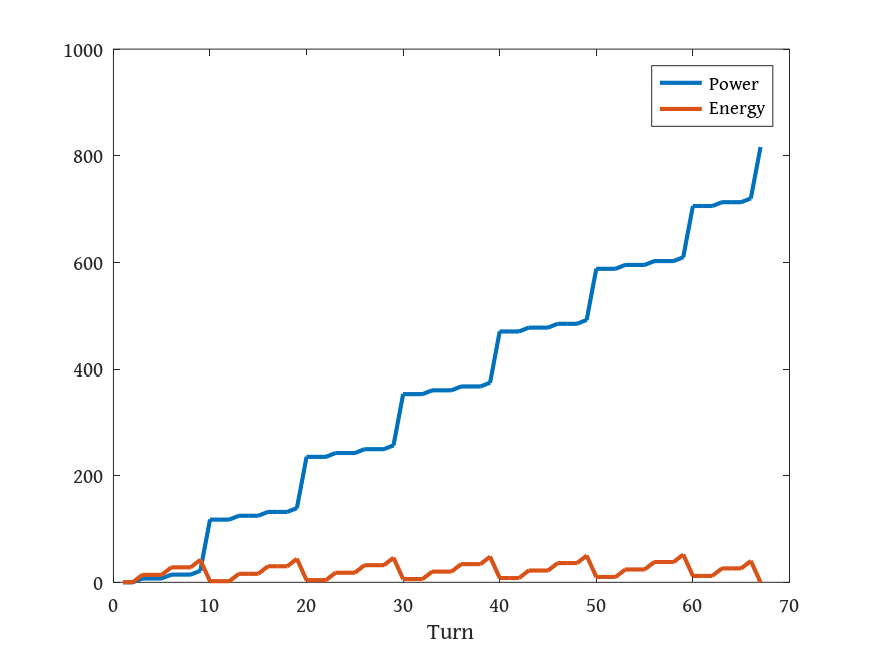
\includegraphics[width=\textwidth]{octave/greninja.png}
  \caption[Damage cycle]{Water Shuriken + Hydro Cannon (7 round cycle, 67 turns)}
\end{figure}

If we expand over multiple cycles of Fast and Charged Attack, we can
 generalize to situations with excess Energy. We know $E_{Charged} \times
 E_{Fast}$ will be a multiple of both the generated and consumed Energy, so
 simply consider $E_{Charged}$ cycles, each of which throws an average of
 $\frac{E_{Charged}}{E_{Fast}}$ Fast Attacks followed by one Charged Attack.

\[ P_{cycles} = E_{Charged} \times (\frac{E_{Charged}}{E_{Fast}} \times P_{Fast} + P_{Charged}) \]

 The number of Fast Attacks in a cycle is actually always either
 $\lfloor\frac{E_{Charged}}{E_{Fast}}\rfloor$
 or $\lceil\frac{E_{Charged}}{E_{Fast}}\rceil$ (iff $E_{Charged}$ is a multiple of
 $E_{Fast}$, these two expressions are equal, and the number of Fast Attacks
 per Charged Attack is constant). Normalize for the total time:

\[ F_{cycles} = \frac{P_{cycles}}{E_{Charged} \times (\frac{E_{Charged}}{E_{Fast}} \times T_{Fast} + T_{Charged})} \]

This has only exacerbated one of the problems we mentioned before: we may
  not get to throw all these Attacks!
Suppose we have some constant chance $0 < L_{KO} \leq 1$ of being knocked out or
 substituted following each Attack we launch, the probability of being
 in to throw the $N$th Attack is $(1 - L_{KO})^{N-1}$.
We could thus define an expected damage from Attack $N$:

\[ E_D(N) = \overline{P} \times (1 - L_{KO})^{N-1} \]

and a cumulative expected damage through $N$ Attacks:

\[ E_{TD}(N) = \sum^N_{i=1} \overline{P} \times (1 - L_{KO})^{i-1} \]

This is a geometric series where $a = \overline{P}$ and $r = 1 - L_{KO}$.
Since $0 \leq r < 1$, this series converges to

\[ E_{TD}(\infty) = \sum^\infty_{i=1} \overline{P} \times r^{i-1} = \frac{\overline{P}}{1 - L_{KO}} \]

Of course, our chance of being knocked out is usually not constant across
 Attacks, but rather an immediate function of our remaining HP and any
 damage we are about to absorb.

\section{Breakpoints}
\label{sec:breakpoints}
